\section{Theoretische Grundlage}
\label{sec:Theorie}
Der Zeemaneffekt beschreibt die Aufspaltung von Spektrallinien im Magnetfeld, sowie die Polarisation des Lichtes. Dabei wird zwischen dem normalen und dem anomalen Zeemaneffekt differenziert. Im folgenden wird die theoretische Grundlage des Versuches skizziert.

\subsection{Magnetisches Moment eines Elektrons}
Elektronen besitzen sowohl einen Bahndrehimpuls $\vec{l}$ sowie einen Eigendrehimpuls $\vec{s}$. In der weiteren Betrachtung werden nur die Drehimpulse der äußeren Schalen der Atome betrachtet, da die der abgeschlossenen Schalen in Summe verschwinden. Ausgehend von der Eigenwertgleichung der Zustände des Atoms werden die Beträge der Quantenzahlen zu
\begin{eqnarray}
  |\vec{l}| = \sqrt{l(l+1)} \hbar  \\
  |\vec{s}| = \sqrt{s(s+1)} \hbar
  \label{eqn:betQua}
\end{eqnarray}
berechnet. Dabei laufen der Bahndrehimpuls $l$ von 0, 1, \ldots $\,$ n-1 und der Spin $s$ ist $\frac{1}{2}$. Für die Berechnung der magnetischen Momente wird das Bohrsche Magneton $\mu_\text{B}$ eingeführt, welches eine Art infinitesimales magnetisches Moment ist. Es entspricht dem magnetischen Moment welches ein Elektron mit $l$=1 erzeugt. Das in Maßeinheiten des Magnetons berechnete magnetische Moment des Bahndrehimpulses beträgt
\begin{equation}
  \vec{\mu_\text{L}} = -\mu_\text{B} \sqrt{l(l+1)} \vec{l_\text{e}} \ .
  \label{eqn:magL}
\end{equation}
Bei der Einführung des magnetischen Momentes des Spins $\mu_\text{s}$
\begin{equation}
  \vec{\mu_\text{s}} = - \mu_\text{B} g_\text{S} \sqrt{s(s+1)} \vec{s_\text{e}}
  \label{eqn:magS}
\end{equation}
tritt der Landé-Faktor $g_\text{S}$ auf, auf welchen im folgenden noch weiter eingegangen wird.

\subsection{Wechselwirkungen der Drehimpulse untereinander}
Bei den Wechselwirkungen der einzelnen Drehimpulse untereinander wird zwischen zwei Fällen unterschieden, die fließend ineinander übergehen. Bei dem ersten Fall wird davon ausgegangen, dass die Kernladungszahl niedrig ist. Die Wechselwirkungen zwischen den einzelnen $\vec{l_\text{i}}$ ist so groß, dass ein Gesamtdrehimpuls $\vec{L}$ eingeführt werden kann.
\begin{equation}
  \vec{L} = \sum \vec{l_\text{i}}
  \label{eqn:L}
\end{equation}
In Analogie zu den einzelnen Drehimpulsen wird das magnetische Moment
\begin{equation}
  |\mu_\text{L}| = \mu_\text{B} \sqrt{L(L+1)}
  \label{magL}
\end{equation}
des Gesmatbahndrehimpuls eingeführt. Analog zum Bahndrehimpuls wird sowohl eine Gesamtspinquantenzahl $\vec{S}$ als auch ein magnetisches Moment $\mu_\text{S}$ eingeführt. Für nicht zu groß Magnetfelder lässt sich der Gesamtdrehimpuls $\vec{J}$ aus der Summe von $\vec{L}$ und $\vec{S}$ einführen. Für den Fall, dass die Wechselwirkungen zwischen Spin und Bahndrehimpuls untereinander vernachlässigt wird, wird von LS-Kopplung gesprochen.
Der zweite Fall der Kopplung von Spin und Bahndrehimpuls wird als j-j-Kopplung bezeichnet. Dabei wird angenommen, dass bei schweren Atomen die Wechselwirkung des Spins und des Bahndrehimpulses eines Elektrons untereinander so groß wird, dass diese nicht mehr vernachlässigt werden kann. Somit müssen die einzelnen Gesamtdrehimpulse
\begin{equation}
  \vec{j_\text{i}} = \vec{l_\text{i}} + \vec{s_\text{i}}
  \label{eqn:j}
\end{equation}
berücksichtigt werden, sodass der Gesamtdrehimpuls $\vec{J}$ die Summe der einzelnen $\vec{j_\text{i}}$ ist.

\subsection{Aufspaltung der Energieniveaus}
Das magnetische Moment des Gesamtdrehimpulses ist die Summe der magnetischen Momente des Spins $\mu_\text{s}$ und des Bahndrehimpulses $\mu_\text{l}$.
\begin{equation}
  \mu = \mu_\text{s} + \mu_\text{l}
\end{equation}
Da der Landé-Faktor bei Elektronen, welche ein Spin $\frac{1}{2}$ haben, in etwa den Wert 2 besitzt, zeigen $\vec{\mu}$ und $\vec{J}$ im Regelfall nicht in die gleiche Richtung. Dies hat zur folge, dass das magnetische Moment in einen Anteil welcher sich parallel zum Gesamtdrehimpuls befindet $\vec{\mu}_\text{J}$ und einem welcher sich senkrecht $\vec{\mu_{\perp}}$ zum Gesamtdrehimpuls befindet zerlegt werden kann. Für die Messzeiten präzidiert der senkrechte Anteil $\vec{\mu_\text{\perp}}$, so schnell um den Gesamtdrehimpuls $\vec{J}$ herum, dass das $\vec{\mu_{\perp}}$ im zeitlichen Mittel wegfällt. Für den Betrag von $\vec{\mu_\text{J}}$ ergibt sich
\begin{equation}
  |\vec{\mu_\text{J}}| = \mu_\text{B} g_\text{J} \sqrt{J(J+1)} \ ,
  \label{eqn:muJ}
\end{equation}
wobei $g_\text{J}$ der Landé-Faktor des Atoms ist. Dieser ist definiert als
\begin{equation}
  g_\text{J} = \frac{3J(J+1) + S(S+1) -L(L+1)}{2J(J+1)}
  \label{eqn:Lan}
\end{equation}
Im folgenden wird angenommen, dass ein äußeres B-Feld in Z-Richtung anliegt. Die Richtungsquantelung besagt, dass bei angelegtem Magnetfeld nur solche Winkel auftreten, bei denen die Projektion von $\mu_\text{J}$ auf das B-Feld ein ganzzahliges vielfaches von $g_\text{J} \mu_\text{B}$ sind.
\begin{equation}
  \vec{\mu_\text{J,z}} = -m g_\text{J} \mu_\text{B}
  \label{eqn:mu}
\end{equation}
Dabei kann die Orientierungsquantenzahl $m$ die Werte $(-J, \cdots, J)$ annehmen. Somit spalten sich die Energieniveaus im Magnetfeld in $2J+1$ Niveaus auf, deren Energiedifferenzen zum magnetfeldfreien Niveau
\begin{equation}
  \Delta E_\text{mag} = m \mu_\text{B} g_\text{J} \text{B}
  \label{eqn:delE}
\end{equation}
ist. Ein Beispiel für die Aufspaltung eines Niveaus mit $J=2$ ist in Abbildung (\ref{fig:Eniv}) zu sehen.
\begin{figure}
  \centering
  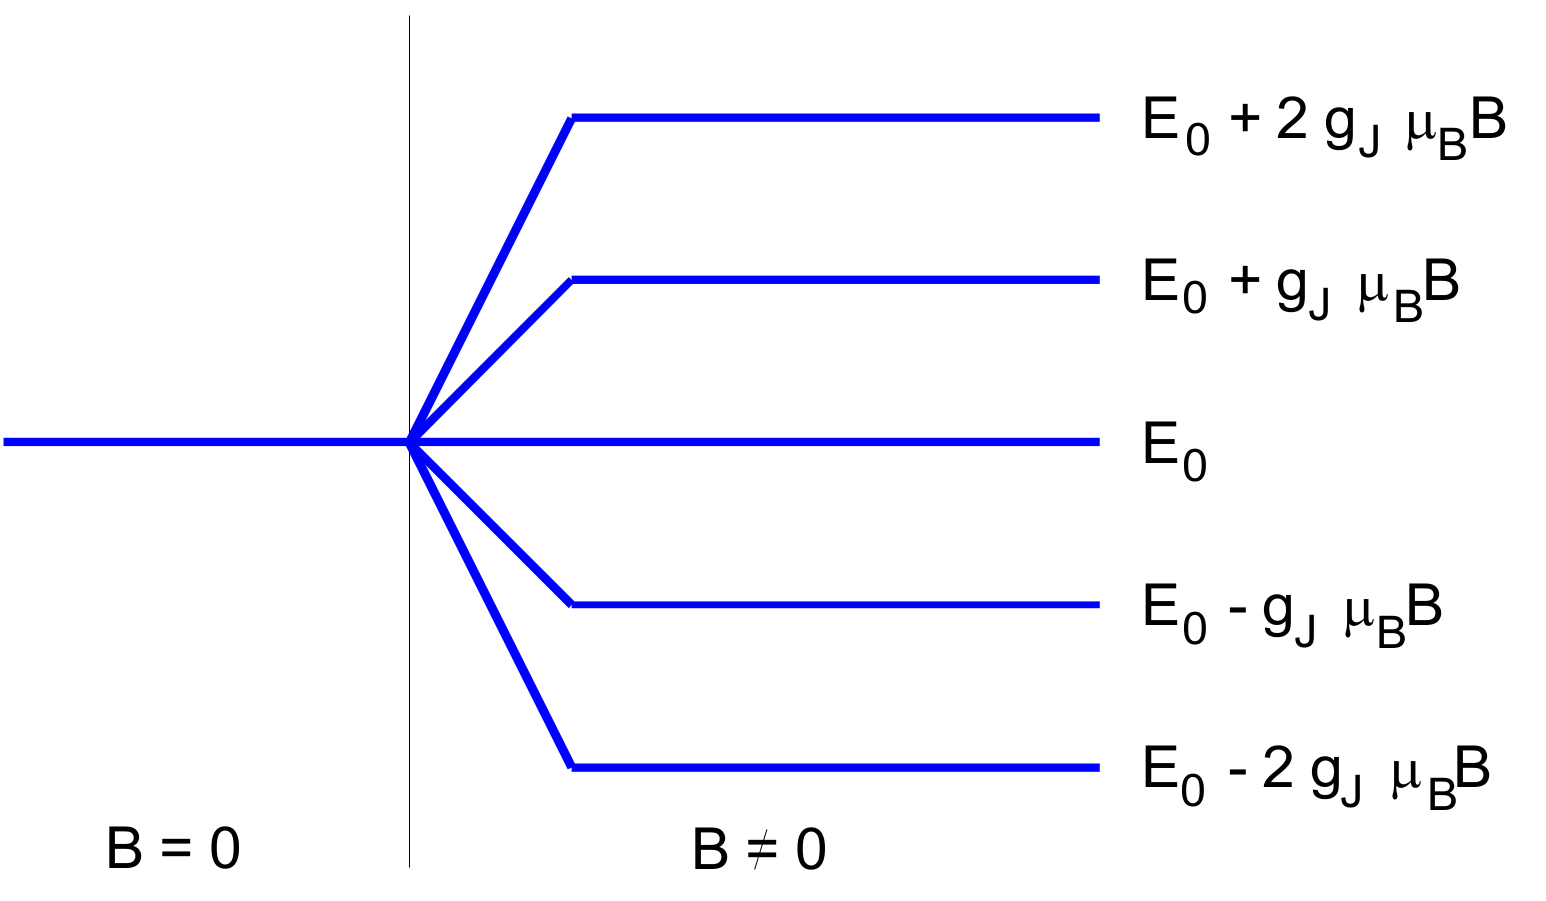
\includegraphics[height=6cm]{./Bilder/ENiveaus.png}
  \caption{Aufspaltung der Energieniveaus im Magnetfeld \cite{V27}}
   \label{fig:Eniv}
\end{figure}

\subsection{Auswahlregeln}
Mithilfe der Schrödingergleichung wird untersucht, welche Niveauübergänge möglich sind. Als Ansatz zur Lösung wird die Summe zweier ebener Wellen genommen, bei denen der Spin berücksichtigt wird. Aus der Dichtefunktion lässt sich die Schwingungsfrequenz $\nu_{\alpha\beta}$ von
\begin{equation}
  \nu_{\alpha\beta}= \frac{E_{\alpha} - E_{\beta}}{\hbar}
  \label{eqn:nu}
\end{equation}
herleiten. Zur Berechnung des Dipolmomentes muss das Integral
\begin{equation}
  -e_0\, \int x \, \Psi^* \Psi \, \text{dV}
\end{equation}
gelöst werden. Anhand der Lösung kann aus dem Poyntingvektor abgeleitet werden, dass alle Beiträge verschwinden, außer wenn $m$ die Zahlenwerte
\begin{equation}
  \Delta m = -1,0,1
\end{equation}
annimmt. Aus der Herleitung lässt sich schließen, dass bei Anlegung eines äußeren magnetischen Feldes für $m = 0$ das elektrische Feld des Lichtes $E_\text{Licht}$ entlang des B-Feldes ausgerichtet ist. Dieser Übergang wird $\pi$ Übergang genannt und ist nur in voller Intensität bei Betrachtung senkrecht zum $\vec{\text{B}}$-Feld (``transversal'') zu beobachten. \\
Ist die Orientierungsquantenzahl $m = \pm 1$, ist das E-Feld um die B-Feldachse zirkular polarisiert. Dieser Übergang wird $\sigma^{+/-}$ genannt, entsprechend des Vorzeichens von $m$ und kann aufgrund der zirkularen Polarisation sowohl longitudinal, als auch transversal beobachtet werden. 

\begin{figure}[H]
  \centering
  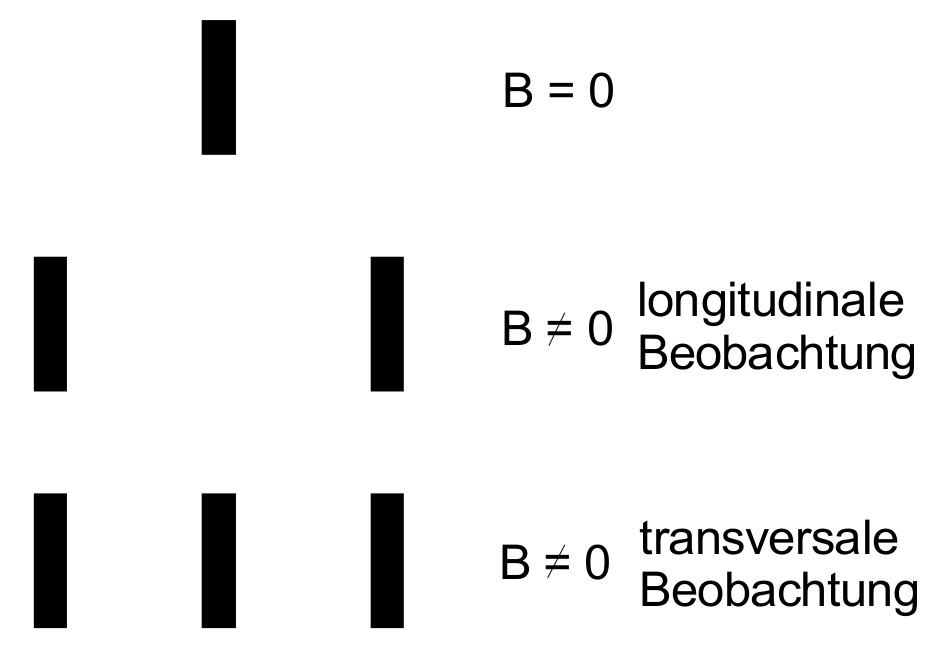
\includegraphics[width=0.8\textwidth]{./Bilder/Aufspaltung.png}
  \caption{Longitudinale und transversale Aufspaltung des Zeemaneffektes bei Anlegung eines äußeren B-Feldes \cite{V27}}
  \label{fig:aufZe}
\end{figure}
Der Abbildung \ref{fig:aufZe} ist zu entnehmen das zur Identifizierung des $\pi$ Übergangs transversal beobachtet wird. Zur Betrachtung des $\sigma$ Übergangs wird zweckmäßger Weise, die longitudinale Beobachtung gewählt. 
\subsection{Normaler Zeeman-Effekt}
Beim normalen Zeeman-Effekt verschwindet die Summe der einzelnen Spins ($S=0$), sodass der entsprechende Landé-Faktor, unabhängig von allen Quantenzahlen $L$ und $J$, $g_\text{J} = 1$ ist. Die Energiedifferenz der Übergänge kann mittels Formel \ref{eqn:delE} berechnet werden. Das Linenspektrum spaltet somit in $2 J + 1$ Linien auf. Eine Aufspaltung der Spektrallinie für $J = 2$ ist in Abbildung \ref{fig:Eniv} zu sehen.
Die Übergänge des Linienspektrum unterliegen den Auswahlregeln, sodass lediglich 3, die $\sigma^{+/-}$ und $\pi$, Übergänge wie in Abbildung \ref{fig:adf} dargestellt detektierte werden können. Dieses Übergänge werden werden ``Triplett'' genannt und ebenfalls beim anomalen Zeeman-Effekt gemessen. Beim anomalen Zeeman-Effekt kann es jedoch zur Aufspaltungen der $\sigma$-Übergänge kommen.
\begin{figure}[H]
  \centering
  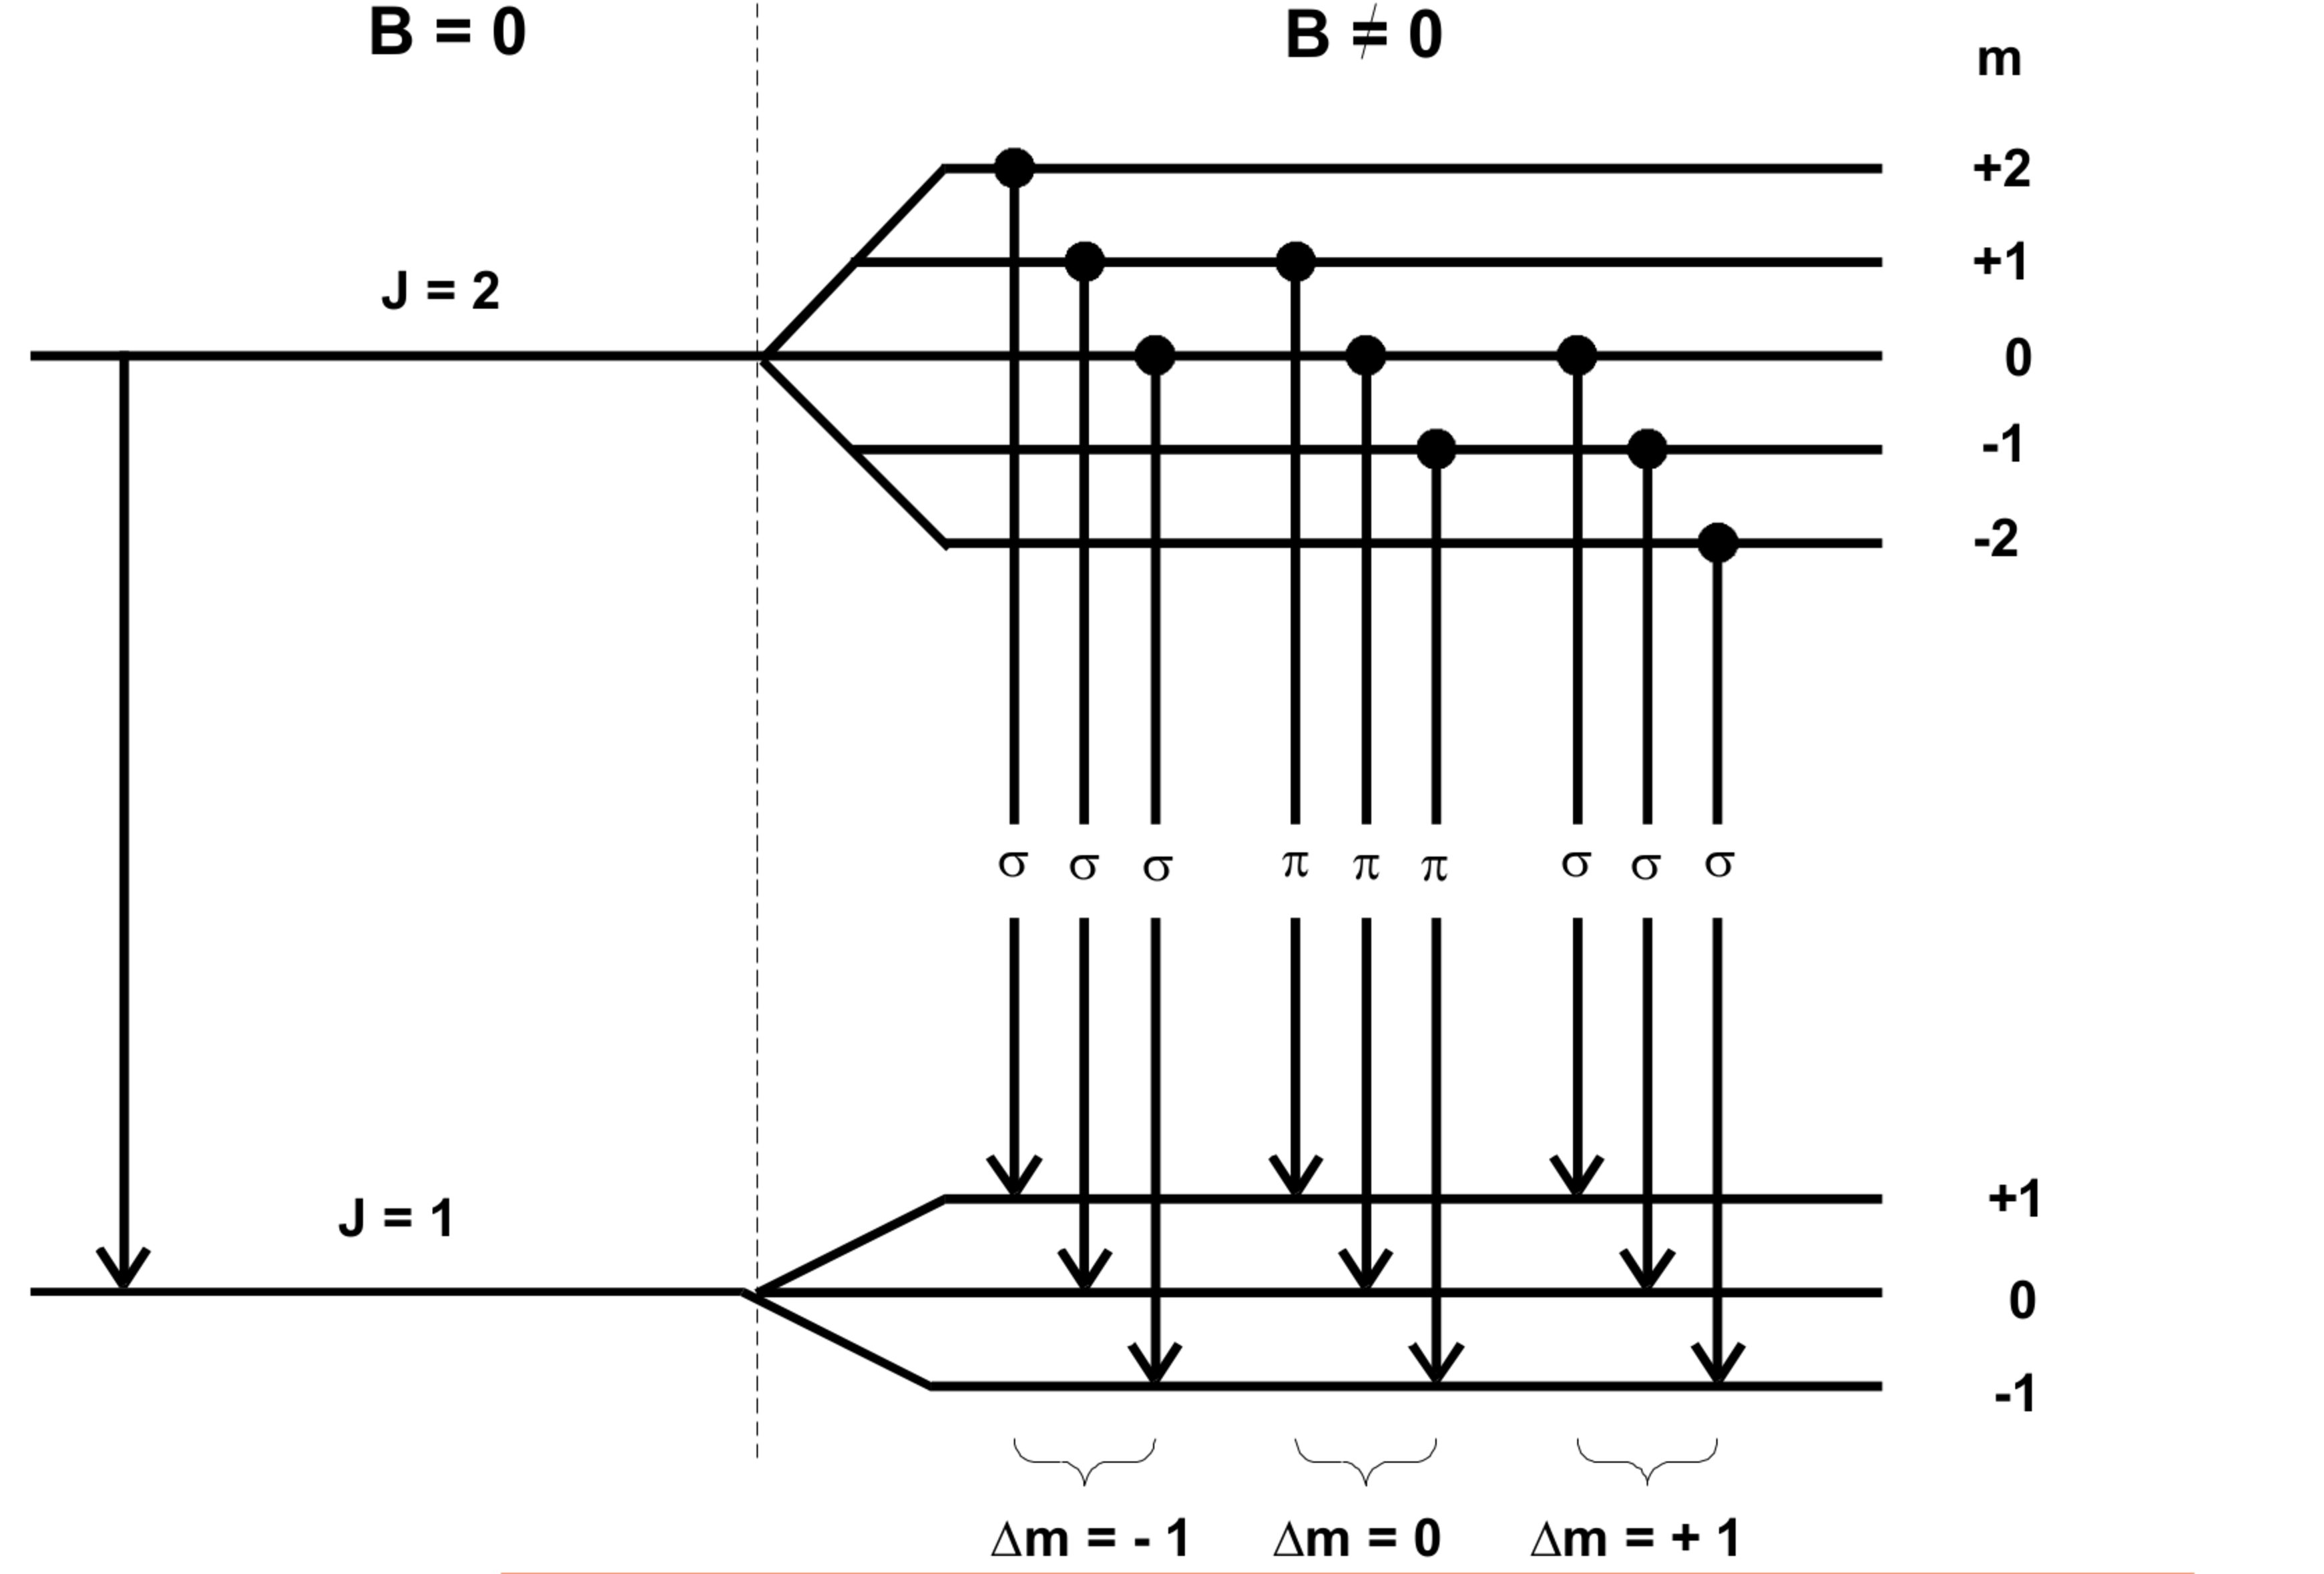
\includegraphics[width=0.6\textwidth]{./Bilder/asd.pdf}
  \caption{$\pi$ und $\sigma$ Übergänge beim normalen Zeeman-Effekt \cite{V27}}
  \label{fig:adf}
\end{figure}

\subsection{Anomaler Zeeman-Effekt}
Bei der Aufspaltung von Spektrallinien im Magnetfeld, bei denen mindestens einer der beiden Zustände einen von Null verschiedenen Gesamtspin hat, wird vom anomalen Zeeman-Effekt gesprochen. Den anomalen Zeemaneffekt kennzeichnet, dass Landefaktoren auftreten, welche ungleich eins sein können. Die Energiedifferenz der einzelnen Niveaus lässt sich durch die Formel
\begin{equation}
  \Delta E = \mu_\text{B}\,B\,(m_1 g_1 - m_2 g_1)
  \label{eqn:dE}
\end{equation}
berechnen. Da die Landefaktoren von L, J und S abhängen gibt es in der Regel mehr als 3 Übergänge zwischen den Energieniveaus die detektiert werden können.

\subsection{Fehlerrechnung}
Sämtliche Fehlerrechnungen werden mit Hilfe von Python 3.4.3 durchgeführt. \\
Für die Berechnung der Mittelwerte wird die Funktion "mean" und für die Standardabweichung die Funktion ``std''aus dem Numpy Paket genutzt. Für die Fehlerfortpflanzung wird die Funktion "ufloat" aus dem Paket "uncertainties \cite{uncertainties}" benutzt. \\
Als Fitfunktion wird "scipy.optimize.curve\_fit \cite{scipy}" verwendet.
